% !TeX root = ../main.tex
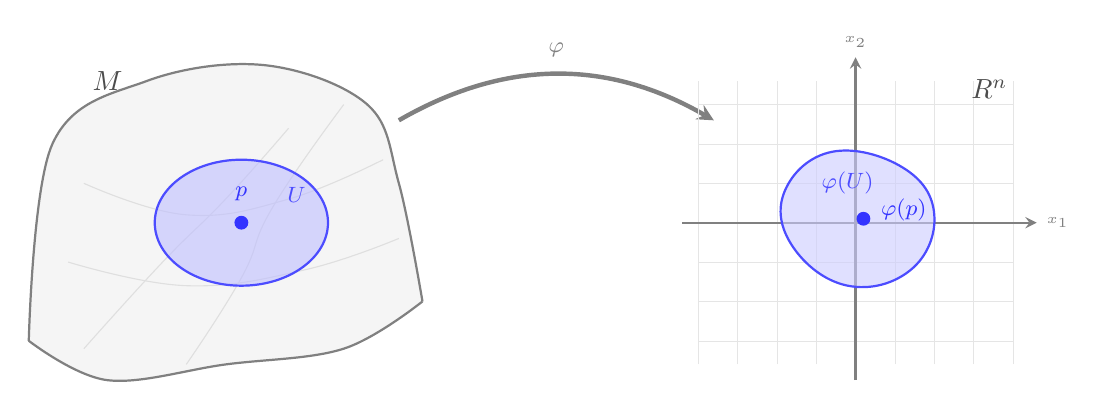
\begin{tikzpicture}[>=stealth, scale=1.0, every node/.style={font=\small}]

% =============================================
% IZQUIERDA: Variedad Topológica M
% =============================================
\begin{scope}[shift={(-4,0)}]
    % Superficie curva (simulada con un path suave)
    \fill[gray!8] 
        plot[smooth, tension=0.6] coordinates {(-2.5,-1.5) (-1.5,-2) (0,-1.8) (1.5,-1.6) (2.5,-1)}
        -- plot[smooth, tension=0.6] coordinates {(2.5,-1) (2.2,0.5) (1.8,1.5) (0.5,2) (-1,1.8) (-2.2,1) (-2.5,-1.5)};
    \draw[black!50, thick] 
        plot[smooth, tension=0.6] coordinates {(-2.5,-1.5) (-1.5,-2) (0,-1.8) (1.5,-1.6) (2.5,-1)};
    \draw[black!50, thick] 
        plot[smooth, tension=0.6] coordinates {(2.5,-1) (2.2,0.5) (1.8,1.5) (0.5,2) (-1,1.8) (-2.2,1) (-2.5,-1.5)};
    
    % Líneas de curvatura (dan profundidad)
    \draw[gray!25, thin] 
        plot[smooth, tension=0.8] coordinates {(-1.8,-1.6) (-0.8,-0.5) (0,0.3) (0.8,1.2)};
    \draw[gray!25, thin] 
        plot[smooth, tension=0.8] coordinates {(-0.5,-1.8) (0.2,-0.7) (0.6,0.2) (1.5,1.5)};
    \draw[gray!25, thin] 
        plot[smooth, tension=0.7] coordinates {(-2.0,-0.5) (-0.5,-0.8) (1.0,-0.6) (2.2,-0.2)};
    \draw[gray!25, thin] 
        plot[smooth, tension=0.7] coordinates {(-1.8,0.5) (-0.5,0.1) (0.8,0.3) (2.0,0.8)};
    
    % Vecindad U (elipse resaltada sobre la superficie)
    \fill[blue!25, opacity=0.6] (0.2,0) ellipse (1.1 and 0.8);
    \draw[blue!70, thick] (0.2,0) ellipse (1.1 and 0.8);
    
    % Punto p
    \fill[blue!80] (0.2,0) circle (2.5pt);
    \node[font=\footnotesize, blue!80, anchor=south] at (0.2,0.15) {$p$};
    
    % Etiqueta U
    \node[font=\footnotesize\bfseries, blue!70] at (0.9,0.35) {$U$};
    
    % Etiqueta M
    \node[font=\bfseries, black!70] at (-1.5,1.8) {$M$};
\end{scope}

% =============================================
% FLECHA DE MAPEO φ
% =============================================
\draw[->, ultra thick, black!50, >=stealth] (-1.8, 1.3) to[bend left=30] node[above, font=\footnotesize\bfseries, yshift=2pt] {$\varphi$} (2.2, 1.3);

% =============================================
% DERECHA: Espacio Euclidiano R^n
% =============================================
\begin{scope}[shift={(4,0)}]
    % Cuadrícula plana
    \draw[gray!20, very thin] (-2,-1.8) grid[step=0.5] (2,1.8);
    
    % Ejes
    \draw[->, thick, black!50] (-2.2,0) -- (2.3,0) node[right, font=\tiny] {$x_1$};
    \draw[->, thick, black!50] (0,-2) -- (0,2.1) node[above, font=\tiny] {$x_2$};
    
    % Imagen de la vecindad φ(U) (mancha deformada)
    \fill[blue!20, opacity=0.6] 
        plot[smooth cycle, tension=0.7] 
        coordinates {(-0.9,0.4) (-0.3,0.9) (0.6,0.7) (1.0,0.1) (0.7,-0.6) (-0.1,-0.8) (-0.8,-0.3)};
    \draw[blue!70, thick] 
        plot[smooth cycle, tension=0.7] 
        coordinates {(-0.9,0.4) (-0.3,0.9) (0.6,0.7) (1.0,0.1) (0.7,-0.6) (-0.1,-0.8) (-0.8,-0.3)};
    
    % Punto φ(p)
    \fill[blue!80] (0.1,0.05) circle (2.5pt);
    \node[font=\footnotesize, blue!80, anchor=south west] at (0.2,-0.1) {$\varphi(p)$};
    
    % Etiqueta φ(U)
    \node[font=\footnotesize\bfseries, blue!70] at (-0.1,0.5) {$\varphi(U)$};
    
    % Etiqueta R^n
    \node[font=\bfseries, black!70] at (1.7,1.7) {$\mathbb{R}^n$};
\end{scope}

\end{tikzpicture}
